\chapter{Theory}
\label{cha:theory}

This chapter introduces relevant theory and related work 

% describe how animal vision translates to camera vision?
% animals have a large field of view, but also require foveated vision: processing is expensive.
% computers do not naturally have this constraint and most CV algorithms do not use foveated vision
% (although visual attention models exist)

\section{Visual Search}


Visual search is a perceptual task which involves seeking out targets among distractors. Eckstein (2011)~\cite{eckstein_visual_2011} identifies four factors that limit performance of visual search in animals:

\begin{itemize}
    \item Foveated vision.
    \item Variability in visual environment and uncertainty about target parameters.
    \item Stochasticity of neural processing.
    \item Limitations of covert attention and memory.
\end{itemize}

The brain utilizes a set of strategies to optimize visual search performance:

\begin{itemize}
    \item Calculation of the visibility of different regions (saliency).
    \item Knowledge about the visual properties of the environment, including targets, distractors and noise.
\end{itemize}

There are a set of statistical regularities that reduce uncertainty of the target location:

\begin{itemize}
    \item Target probabilities varying across locations and predictive cues.
    \item Contextual cuing
\end{itemize}


Interestingly, studies in humans have shown

\begin{itemize}
    \item We do not use memory during visual search
    \item We have easier to differentiate unknown distractors from targets (or vice versa?) 
\end{itemize}

% https://www.nature.com/articles/s41598-021-86669-2


% Bayesian observer: https://www.nature.com/articles/nature03390.pdf

An alternative model of visual search is \textit{guided search} by Wolfe (2021). 
% Guidance summary section
% Scene guidance section
% Meaning map (Henderson and Hayes, 2017): representation akin to salience map that reflects bottom-up guidance of attention.
% To create a meaning map, scenes are divided into many small regions. Observers were asked to rate meaningfulness of each patch (an eye might be meaningful while a wall is not).
% This forms a heatmap of meaningfulness. These have turned out to predict eye movements better than salience maps calculated for the same images  (Pedziwiatr, Wallis, Kümmerer, & Teufel, 2019).
% Syntactic (physics of objects in the scene, toasters don't float) vs. semantic guidance (meaning of objects in the scene, toasters don't belong in the bathroom).

Wolfe also presents a simulation of the model. Simulates some mechanics of the search


\subsection{Active Vision}

Much of current research in computer vision studies problems with passive observers where images are passively sampled. The problem considered in this project contains an \textit{active vision}~\cite{aloimonos_active_1988} system. The observer (agent) can manipulate the viewpoint of the camera in order to investigate the environment and get better information from it. This closer to human perceptual activity which is both exploring and searching. A study of basic problems of vision shows that active vision systems have several computational advantages over passive ones for common perceptual tasks~\cite{aloimonos_active_1988}. % relevant?

% active object detection

\section{Reinforcement Learning}

Reinforcement learning (RL) is a subfield of machine learning concerned with learning from interaction how to achieve a goal. An \textit{agent} and its \textit{environment} interact continually over discrete time steps. At each time step the agent selects some \textit{action} that updates the state of the environment, and gives it a \textit{reward}. The agent selects actions using a stochastic \textit{policy} with the goal of maximizing the \textit{return} which is usually defined as the discounted sum of future rewards.

\subsection{Markov Decision Process}

The RL setup is usually formalized as a (finite) Markov decision process (MDP).

The problem of learning from interaction to achieve a goal is usually framed as a (finite) Markov Decision Process (MDP). For regular MDPs it is assumed that the learning agent has access to some representation of the underlying \textit{state} of the environment which it uses to select \textit{actions}. For many problems this is not true. A partially observable Markov decision process (POMDP) is a generalization of an MDP in which it is assumed that the environment has some well defined underlying latent state, but the agent only perceives a partial \textit{observation} of it from the environment. 

A POMDP is formally defined as a 7-tuple \(\langle \mathcal{S}, \mathcal{A}, \mathcal{O}, \mathcal{R}, \mathcal{T}, \Omega, \gamma \rangle\), where

\begin{itemize}
    \item \(\mathcal{S}\) is a finite set of states,
    \item \(\mathcal{A}\) is a finite set of actions,
    \item \(\mathcal{T}\) is a set of conditional state transition probabilities,
    \item \(\mathcal{R} : S \times A \rightarrow \mathbb{R}\) is a reward function,
    \item \(\Omega\) is a finite set of observations,
    \item \(\mathcal{O}\) is a set of conditional observation probabilities, and
    \item \(\gamma \in [0, 1]\) is a discount factor.
\end{itemize}

\begin{figure}
    \centering
    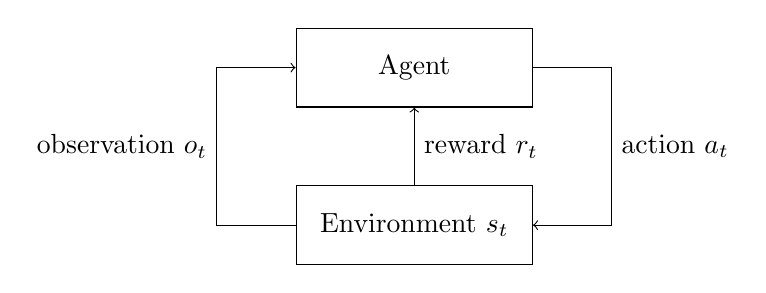
\begin{tikzpicture}[node distance=2cm]
    \tikzstyle{block} = [rectangle,minimum width=3cm,minimum height=1cm,text centered,draw=black,fill=white]
    \node (agent)[block]{Agent};
    \node (environment)[block,below of=agent]{Environment \(s_t\)};
    \draw [->] (agent.east) -- ++(1cm,0) -- node [anchor=west]{action \(a_t\)} ++(0,-2cm) -- (environment.east);
    \draw [->] (environment.north) -- node [anchor=west]{reward \(r_t\)} (agent.south);
    \draw [->] (environment.west) -- ++(-1cm,0) -- node [anchor=east]{observation \(o_t\)} ++(0,+2cm) -- (agent.west);
\end{tikzpicture}
    \label{fig:pomdp}
    \caption{Partially observable Markov decision process.}
\end{figure}

The agent interacts with the environment at discrete time steps \(t = 0, 1, 2, \dots T\). At each time step \(t\), the agent receives an observation of the environment's state \(O_t \in \Omega\) and selects some action \(A_t \in \mathcal{A}\). In the next time step the agent receives a reward

action \(a \in \mathcal{A}\) which causes the environment to transition to state \(s^\prime\) with probability \(\mathcal{T}(s^\prime | s, a)\).
It receives an observation \(o \in \Omega\) with probability \(\mathcal{O}(o | s^\prime, a)\), as well as a reward \(r\) given by \(\mathcal{R}(s, a)\).

This interaction is repeated until the end of the episode at time step \(T\). The goal of the agent is to maximize the \textit{discounted return}, defined as the discounted sum of future rewards \(G_t \doteq \sum_{k=t+1}^T \gamma^{k-t-1} R_{k}\) where \(\gamma\) reflects the uncertainty of the environment.

%An MDP satisfies the Markov property: the process is memoryless. A POMDP is not memoryless, as observations only convey part of the underlying state. However, the \textit{history} \(H_t = A_0, O_1, R_1, \dots, A_{t-1}, O_t, R_t\) does.

Planning in a POMDP is undecidable, and solving them is often computationally intractable. Approximate solutions are more common.

\subsection{Policies and Value Functions}

Most RL algorithms estimate both a \textit{value function} that tells the agent how good it is to be in a given state, and a 

\subsection{Policy Optimization}

This work will focus on policy optimization algorithms.

\subsection{Actor Critic Models}

\subsection{Exploration and Exploitation}

% The thesis could also be called Efficient Exploration
% 

% Go into motivation if we use this

% Custom rewards are often needed
% intrinsic?

\subsection{Generalization}

% reality is dynamic
% agents need to be robust to variation
% capability to transfer and adapt to unseen but similar environments
% most current research works on benchmarks that do not test this (MuJoCo, Arcade learning environment)

% refer to survey
% specifically IID (train_dist = test_dist) and OOD environments (train_dist != test_dist)

% how do they handle training and test set?

Kobbe et al. (2020)~\cite{} study generalization in RL. They introduce a benchmark of procedurally generated i.i.d. environments, and find that this is essential to 


\section{Automating Visual Search}

% CT scan material: there is way less variance, otherwise similar. Big difference is that we look at more variance in many aspects?

% CV material: different in that the object is assumed to be visible

\section{Deep Reinforcement Learning}

Ghesu et al. ()~\cite{ghesu_multi-scale_2019} use XXX